\question La gráfica de la Figura \ref{fig:escuela_pie} muestra la composición de una escuela de 3 200 personas.

\begin{figure}[H]
    \centering
    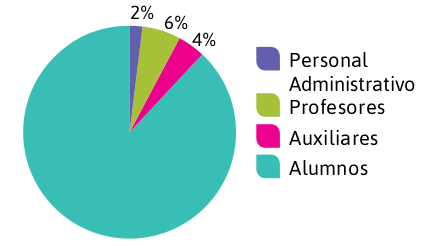
\includegraphics[width=.5\linewidth]{escuela_pie.png}
    \captionof{figure}{Gráfico circular sobre la distribución de los roles en una escuela (en porcentaje).}
    \label{fig:escuela_pie}
\end{figure}
% \begin{minipage}{.45\textwidth}

% \end{minipage}\hfill
% \begin{minipage}{.45\textwidth}
\begin{parts}
    \part[5] ¿Cuántas personas trabajan en la administración?
    \begin{solutionbox}{2cm}
    \end{solutionbox}

    \part[5] ¿Cuántos profesores hay en esa escuela?

    \begin{solutionbox}{2cm}
        Los profesores son el 6\% de 3200, entonces:
        \[\dfrac{6}{100}\times 3200=0.06\times 3200=192\]
    \end{solutionbox}

    \part[5] ¿Cuántas personas son auxiliares?

    \begin{solutionbox}{2cm}
    \end{solutionbox}

    \part[5] ¿Cuál es el porcentaje de alumnos?

    \begin{solutionbox}{2cm}
        El porcentaje de alumnos es::
        \[100\%-2\%-6\%-4\%=88\%\]
    \end{solutionbox}

    \part[5] ¿Cuántos alumnos tiene la escuela?
    \begin{solutionbox}{2cm}
    \end{solutionbox}
\end{parts}
% \end{minipage}
